\PassOptionsToPackage{unicode=true}{hyperref} % options for packages loaded elsewhere
\PassOptionsToPackage{hyphens}{url}
%
\documentclass[]{article}
\usepackage{lmodern}
\usepackage{amssymb,amsmath}
\usepackage{ifxetex,ifluatex}
\usepackage{fixltx2e} % provides \textsubscript
\ifnum 0\ifxetex 1\fi\ifluatex 1\fi=0 % if pdftex
  \usepackage[T1]{fontenc}
  \usepackage[utf8]{inputenc}
  \usepackage{textcomp} % provides euro and other symbols
\else % if luatex or xelatex
  \usepackage{unicode-math}
  \defaultfontfeatures{Ligatures=TeX,Scale=MatchLowercase}
\fi
% use upquote if available, for straight quotes in verbatim environments
\IfFileExists{upquote.sty}{\usepackage{upquote}}{}
% use microtype if available
\IfFileExists{microtype.sty}{%
\usepackage[]{microtype}
\UseMicrotypeSet[protrusion]{basicmath} % disable protrusion for tt fonts
}{}
\IfFileExists{parskip.sty}{%
\usepackage{parskip}
}{% else
\setlength{\parindent}{0pt}
\setlength{\parskip}{6pt plus 2pt minus 1pt}
}
\usepackage{hyperref}
\hypersetup{
            pdftitle={Methods},
            pdfauthor={Chris Adlam},
            pdfborder={0 0 0},
            breaklinks=true}
\urlstyle{same}  % don't use monospace font for urls
\usepackage[margin=1in]{geometry}
\usepackage{graphicx,grffile}
\makeatletter
\def\maxwidth{\ifdim\Gin@nat@width>\linewidth\linewidth\else\Gin@nat@width\fi}
\def\maxheight{\ifdim\Gin@nat@height>\textheight\textheight\else\Gin@nat@height\fi}
\makeatother
% Scale images if necessary, so that they will not overflow the page
% margins by default, and it is still possible to overwrite the defaults
% using explicit options in \includegraphics[width, height, ...]{}
\setkeys{Gin}{width=\maxwidth,height=\maxheight,keepaspectratio}
\setlength{\emergencystretch}{3em}  % prevent overfull lines
\providecommand{\tightlist}{%
  \setlength{\itemsep}{0pt}\setlength{\parskip}{0pt}}
\setcounter{secnumdepth}{0}
% Redefines (sub)paragraphs to behave more like sections
\ifx\paragraph\undefined\else
\let\oldparagraph\paragraph
\renewcommand{\paragraph}[1]{\oldparagraph{#1}\mbox{}}
\fi
\ifx\subparagraph\undefined\else
\let\oldsubparagraph\subparagraph
\renewcommand{\subparagraph}[1]{\oldsubparagraph{#1}\mbox{}}
\fi

% set default figure placement to htbp
\makeatletter
\def\fps@figure{htbp}
\makeatother

\usepackage{wrapfig}
\usepackage{lipsum}

\title{Methods}
\author{Chris Adlam}
\date{}

\begin{document}
\maketitle

\hypertarget{methods}{%
\section{Methods}\label{methods}}

\hypertarget{study-area}{%
\subsection{Study area}\label{study-area}}

Located in the Klamath-Siskiyou mountains of northern California, the
WKRP is a 1.2 million-acre collaborative landscape restoration effort
between the Karuk Tribe, US Forest Service and local NGOs (Harling and
Tripp 2014). The area's main vegetation class is mixed evergreen forest
(Steel, Safford, and Viers 2015). The prevalence of hardwoods and
Douglas-fir (`Pseudotsuga menziesii') distinguish the Klamath-Siskiyou
mixed evergreen forests from those of the Cascade Mountains and Sierra
Nevada (Barbour and Billings 2000; Whittaker 1961). These forests were
historically managed by the Karuk tribe using frequent
(\textasciitilde{}12.5 year interval), low-intensity prescribed burning
(Taylor and Skinner 1998, 2003). One of the main goals of the WKRP is to
restore the fire regimes within the Karuk tribe's aboriginal territory
in a way that promotes the resilience of these ecosystems to high
severity fire and climate change (Harling and Tripp 2014).

\hypertarget{data-collection}{%
\subsection{Data collection}\label{data-collection}}

I conducted surveys at 110 sites varying in time-since-fire and burn
severity (48 sites surveyed in 2018 and 62 in 2019). Sampling sites were
in lower elevation (mean 759m, range 241-1500m) mixed evergreen forest,
with some in transition areas into dry or moist mixed conifer
(classification based on FRID data, Safford and Van de Water (2014)).
The median historic fire return interval in these forests is 13 years
(Van de Water and Safford 2011).

\begin{wrapfigure}{R}{0.5\textwidth}

\hfill{}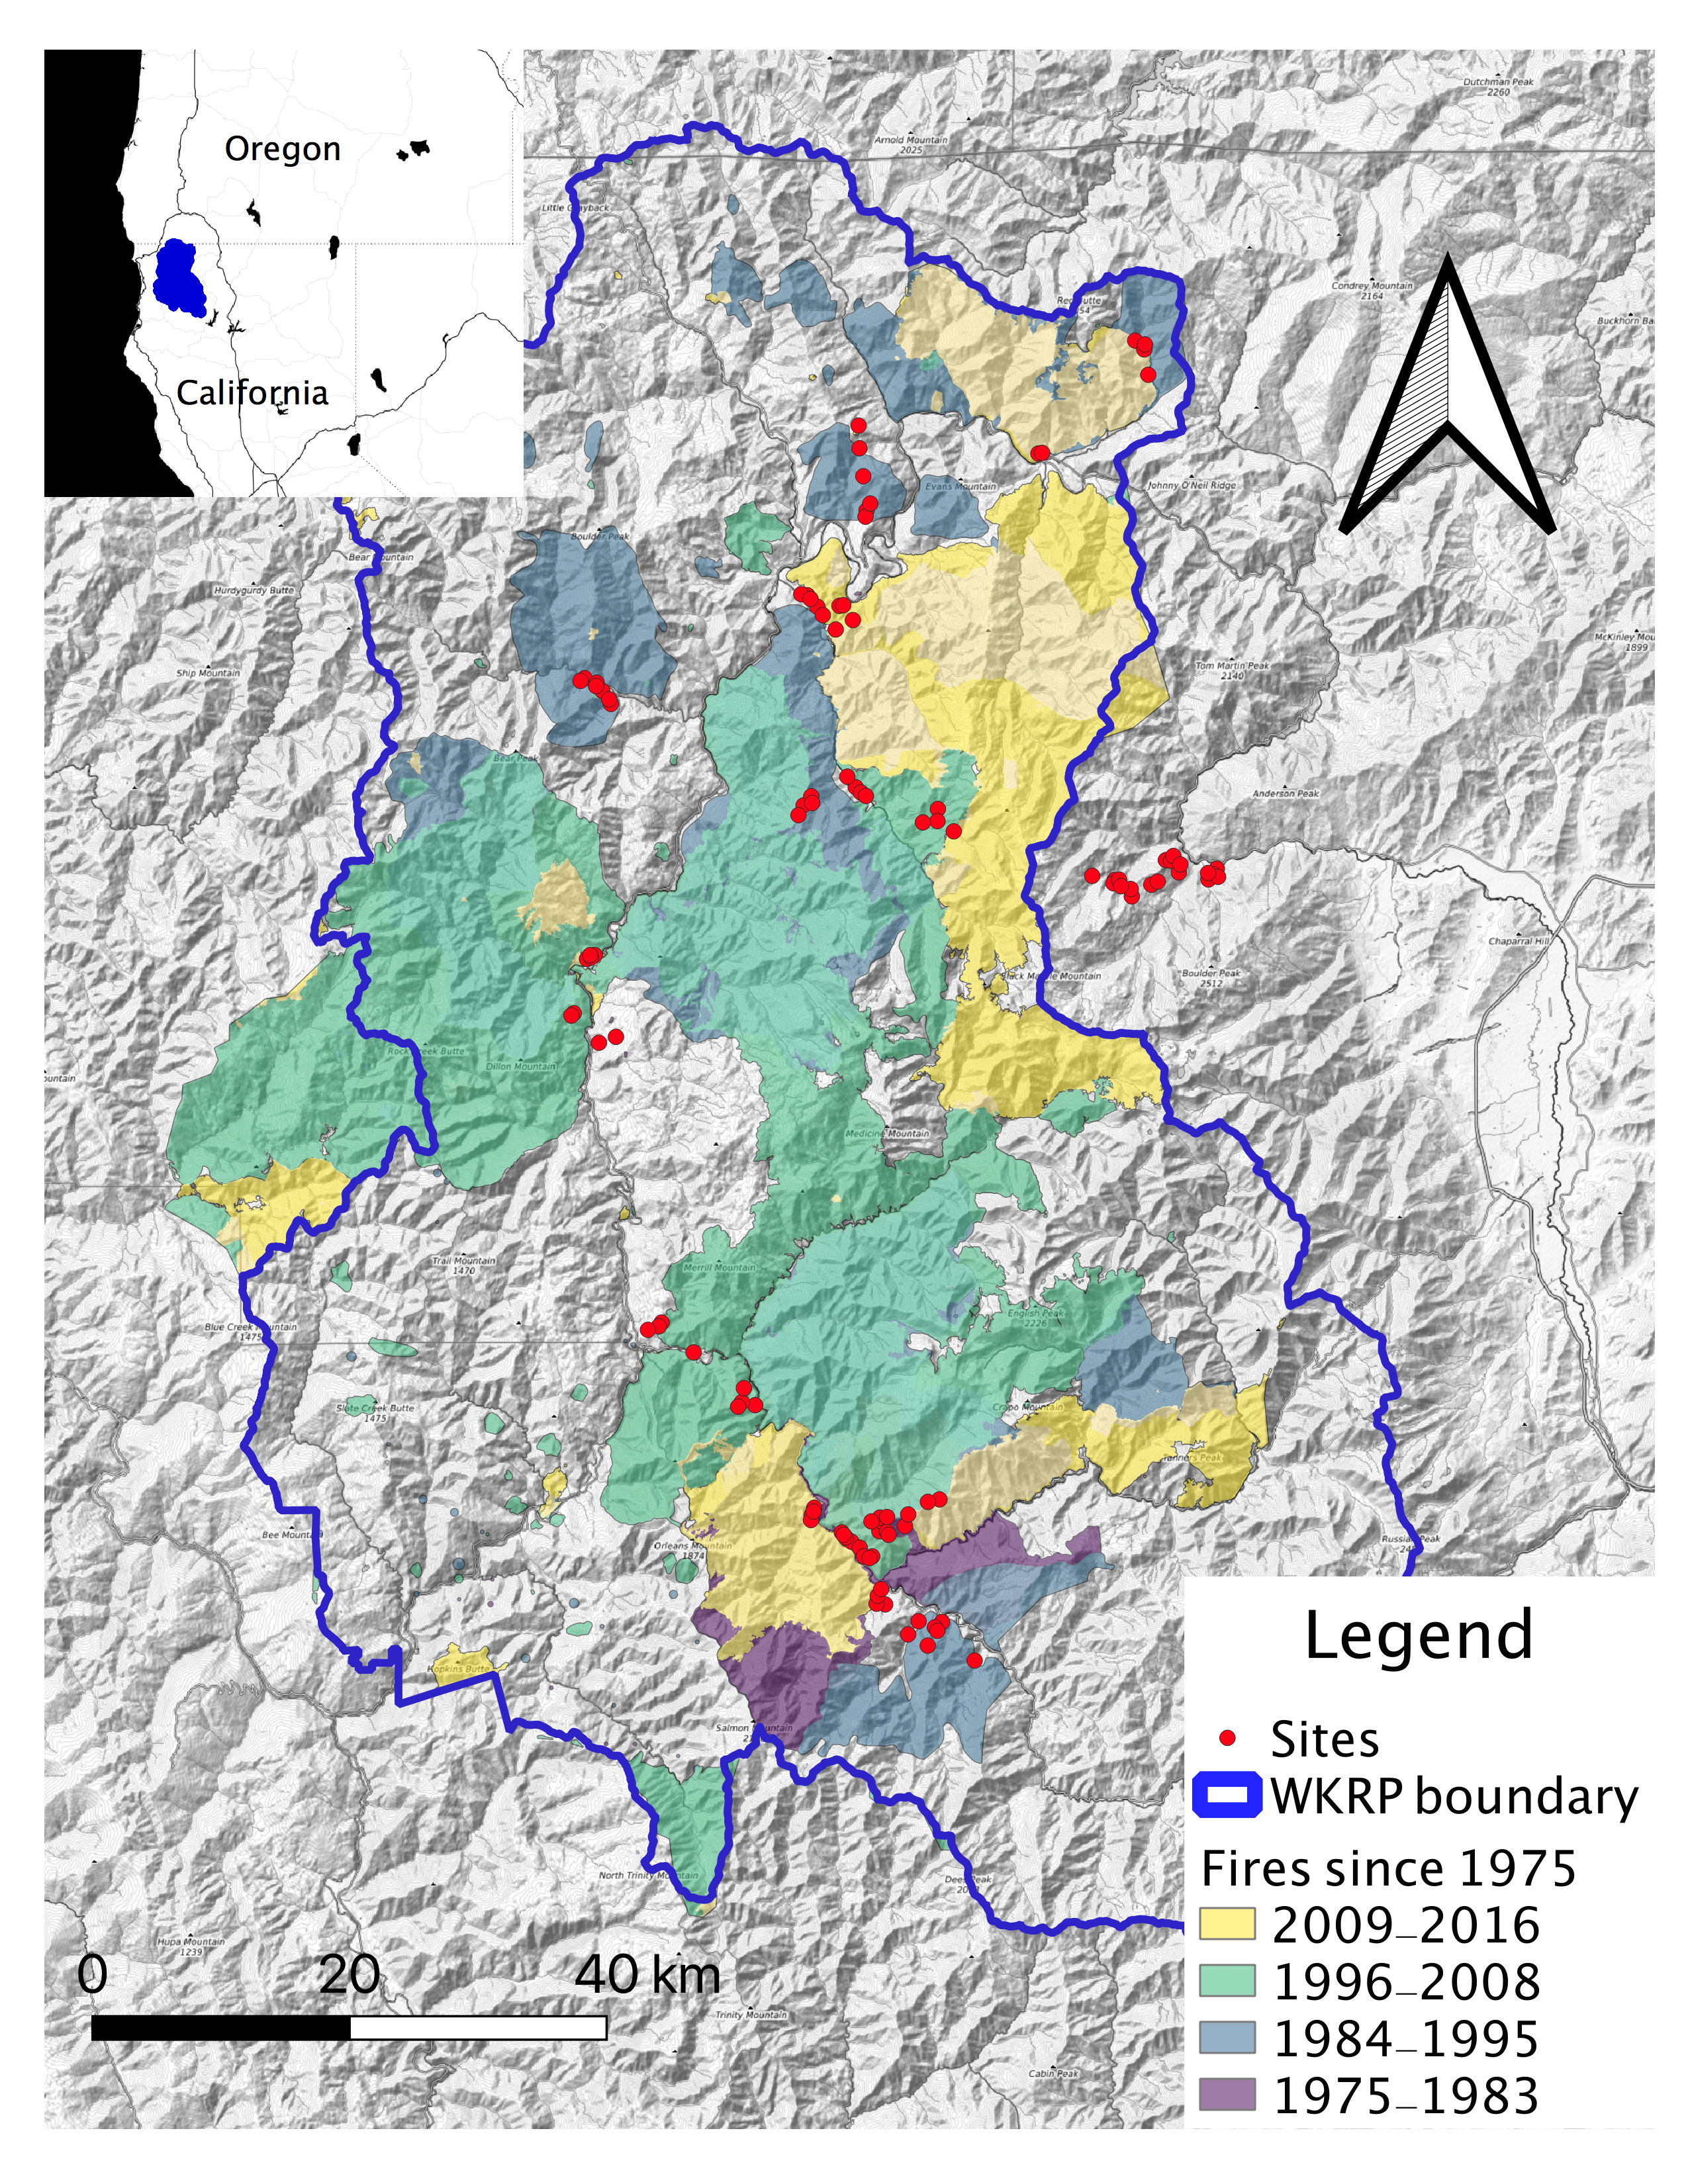
\includegraphics[width=.5\textwidth]{/Users/christopheradlam/Desktop/Davis/R/GitHub Repos/Fire_mosaics/output/WKRP_map} 

\caption{Map of WKRP project area and sampling sites}\label{fig:unnamed-chunk-2}
\end{wrapfigure}

Sampling sites were placed in low severity and high severity burns,
defined respectively as \textless{}25\% canopy mortality and
\textgreater{}75\% canopy mortality (Miller et al. 2009), in
long-unburnt stands (\textgreater{}40 years since last fire), in sites
affected by multiple burns, and sites that were thinned and burnt. At
all burnt sites, time-since-fire varied from 2 to 32 years. Multiple
burns and thinned and burnt sites were placed in areas with intermediate
canopy cover (30-65\% cover). While it is possible for both to still
have high canopy cover (or little canopy), I was only interested in
``treatments'' (active or passive) that reduce canopy cover
significantly. Such canopy reduction corresponds to the level
recommended for understory restoration (Abella and Springer 2015) and
for mitigating the risk of crown fires (Moghaddas et al. 2010). As a
result of this approach, the habitats studied follow a gradient of
canopy cover (Figure 1). Burn severity was evaluated a priori based on
the relative difference normalized burn ratio (Miller and Thode 2007)
and verified in situ by visually estimating the magnitude of canopy
cover reduction. Since the habitats differ mostly by the severity of
fire's impact, I will henceforth refer to different ``severity
categories'' for simplicity, even though this is an imperfect
description of multiple burn and thinned and burnt sites.

Several tests were used to ensure that the differences observed between
site categories were not the product of a climatic or topographic
pattern rather than fire history. To test for climate differences, I
compared the climatic water deficit (CWD, the difference between
potential and actual evapotranspiration). Using the Basin
Characterization Model 30-year average for 1981-2010 (Flint et al.
2013), I found no difference between the severity categories (ANOVA, F =
1.41, p = 0.237). Heat load, which accounts for the effect of slope,
aspect and lattitude on insolation and temperature (McCune and Keon
2002), was not different among categories except that it was slightly
lower for high severity sites (although this might seem
counterintuitive, it is explained by the fact that high severity sites
were steeper on average, and heat load decreases with slope gradient on
north-facing aspects). However, due to the limited availability of
prescribed burn areas, I had to make some concessions in study design.
While there were numerous sites available for the other severity
categories, the only prescribed burn sites that met my criteria for
minimum size, canopy reduction, and absence of other disturbance factors
were located in two project areas. These were higher in elevation on
average than the other severity categories (mean = 1101m, 95\% CL =
965-1237m) and more clustered (average distance among sites
\textless{}10km compared to 28-36km for the other severity categories).
While these factors limit the generalizability of the patterns observed
at these sites, this is a common challenge for studies of prescribed
fires. Therefore I still include the prescribed burn sites in the study
in the hope that my findings can be used in designing more robust future
investigations.

At each site, I recorded aspect, slope, elevation, and canopy cover
(trees over 5m in height, by visual estimation). For all sites, I
surveyed plants, epiphytic lichens, and birds. Presence of all plants
and lichen species was determined in an 11.3m-radius plot following the
Common Stand Exam protocol (Service 2008). Plants were identified using
the Jepson manual (Baldwin et al. 2012) and lichens were identified
using Mccune and Geiser's Macrolichens of the Pacific Northwest (McCune
and Geiser 2009). Only native plant species are included in the
analysis, although exotic species were generally few. Species of some
plant genera were pooled if they shared similar ecological requirements
(eg. \textbf{\emph{Arctostaphylos}}, \textbf{\emph{Cryptantha}},
\textbf{\emph{Pyrola}}). Species of the lichen genera
\textbf{\emph{Usnea}} and \textbf{\emph{Bryoria}} were also pooled
because of he difficulty in differentiating them. I also conducted two
10-minute bird point counts on separate, non-consecutive days. All bird
detections within a 100m radius were recorded. The two hummingbird
species (Anna's and Rufous Hummingbird) were pooled, as were
Black-throated Gray Warblers and Hermit Warblers
(\textbf{\emph{Setophaga}} sp.), because it was not always possible to
differentiate these species without by sound. Lastly, for high severity,
low severity and unburnt sites, I set up a custom-built flight-intercept
trap for flying insects that were left out for two days (Russo et al.
2011).

\hypertarget{analysis}{%
\subsection{Analysis}\label{analysis}}

\hypertarget{species-composition-and-diversity-patterns}{%
\subsubsection{Species composition and diversity
patterns}\label{species-composition-and-diversity-patterns}}

I conducted a PERMANOVA analysis to test the significance of
dissimilarity between the different severity categories (McArdle and
Anderson 2001) using the adonis2() function from the vegan package in R
(Oksanen et al. 2007), with 999 permutations. Then I conducted PERMANOVA
pairwise comparisons between each severity category. To minimize the
risk of making a type-1 error from carrying out multiple pairwise tests
on a single data set, I adjusted the p-values using the Bonferroni
correction method (Rice 1989).

Next, I analyzed patterns of alpha, beta and gamma diversity for plants,
birds, and lichens. Alpha diversity is equivalent to species richness
per plot. I tested for the significance of the difference in richness
between severity categories with anovas and post-hoc Tukey tests using
the R package ``emmeans'' (Lenth et al. 2020). To further evaluate the
influence of canopy cover on species richness, I performed anovas with
plant and bird richness as the response variable and percent tree cover
as the predictor for the lower canopy cover habitat (high severity
burns), intermediate canopy habitats (multiple and thinned and burnt
stands), and higher canopy cover habitats (low severity and unburnt).
This tiered approach was chosen to isolate the effect of treatment and
of canopy cover, since the treatments themselves are the principal
driver of canopy cover differences.

I calculated beta diversity, or the amount of variation in species
composition and richness between sites within each severity category,
using the R package vegetarian v1.2 (Charney and Record, 2009). I used
the Jaccard index (Jost 2007) to represent the extent to which species
are shared in each pair of samples. I compared results between
treatments using standard errors from bootstrapping given by the package
vegetarian.

Because the number of samples in each severity category was unequal,
simply comparing the total number of species found in each severity
category was not an adequate way to evaluate gamma diversity, the size
of the species pool for each habitat. Instead, I generated sample-based
rarefaction curves (Colwell et al. 2012) using package iNEXT v. 2.0.20
(Chao et al. 2014; Hsieh, Ma, and Chao 2016). This method uses Hill
numbers, or effective species numbers based on species richness.
Estimates were interpolated from site-based incidence data to account
for unequal sample sizes (Colwell et al. 2012) and then extrapolated to
twice the size of the smallest sample (Chao et al. 2014). I compared
results between treatments using 95\% confidence intervals from
bootstrapping.

Insects were not sampled in the multiple burns and thinned and burnt
sites, but I include them nevertheless to compare species communities in
the unburnt, low severity and high severity burns. Comparisons of alpha,
beta and gamma diversity were not as meangingful for insects, because of
the small number of taxa (orders or suborders). Instead, I used an
indicator species analysis using the function multipatt() in the package
indicspecies v1.7.8 (De Cáceres and Legendre 2009) to determine which
taxa showed a preference for high severity or low severity and unburnt
stands (the latter were pooled because the PERMANOVA suggested their
community composition did not differ).

Lastly, I wanted to determine if the multiple burns and thinned and
burnt stands tended to contain species affiliated with high severity
burns and/or those associated with low severity and unburnt stands. Four
hypotheses were envisioned: 1) Species associated with high severity
burns are associated with the actively or passively managed stands; 2)
Species associated with unburnt stands and low severity burns are
associated with the actively or passively managed stands; 3) Both of
these species cohorts are found in the actively or passively managed
stands, presumably because they are intermediate in environmental
characteristics such as canopy cover; 4) Neither cohort is found in the
actively or passively managed stands, presumably because the
intermediate canopy cover creates inhospitable conditions for both and
favors a completely different species assemblage. The third hypothesis
would mean that reducing canopy cover for fire management would be
compatible with biodiversity objectives, while the fourth would be the
worst case scenario. To determine which of these four hypothese was
correct, I identified species that prefer high severity burns and
species that prefer unburnt stands and low severity burns by using a
simple criterion: if a species was found twice as frequently in one
habitat than the other, I considered that it exhibited a preference for
that habitat. Only species that occurred in more than five sites (18\%
of the total number of sites) were included. For each cohort (those
found twice as frequently in the high severity burns and those found
twice as frequently in the low severity burns and unburnt stands), I
then determined if it was also found twice as frequently in the multiple
burns and/or thinned and burnt stands. To determine which of the four
hypotheses above was correct, I evaluated the frequency with which
species preferring high severity burns or low severity burns and unburnt
stands also favored the multiple burns and/or thinned and burnt stands.

\hypertarget{refs}{}
\leavevmode\hypertarget{ref-abellaEffectsTreeCutting2015}{}%
Abella, Scott R., and Judith D. Springer. 2015. ``Effects of Tree
Cutting and Fire on Understory Vegetation in Mixed Conifer Forests.''
\emph{Forest Ecology and Management} 335 (January): 281--99.
\url{https://doi.org/10.1016/j.foreco.2014.09.009}.

\leavevmode\hypertarget{ref-baldwinJepsonManualVascular2012}{}%
Baldwin, Bruce G., Douglas H. Goldman, David J. Keil, Robert Patterson,
Thomas J. Rosatti, and Linda Ann Vorobik. 2012. \emph{The Jepson Manual:
Vascular Plants of California}. Univ of California Press.

\leavevmode\hypertarget{ref-barbourNorthAmericanTerrestrial2000}{}%
Barbour, Michael G., and William Dwight Billings. 2000. \emph{North
American Terrestrial Vegetation}. Cambridge University Press.

\leavevmode\hypertarget{ref-chaoRarefactionExtrapolationHill2014}{}%
Chao, Anne, Nicholas J. Gotelli, T. C. Hsieh, Elizabeth L. Sander, K. H.
Ma, Robert K. Colwell, and Aaron M. Ellison. 2014. ``Rarefaction and
Extrapolation with Hill Numbers: A Framework for Sampling and Estimation
in Species Diversity Studies.'' \emph{Ecological Monographs} 84 (1):
45--67. \url{https://doi.org/10.1890/13-0133.1}.

\leavevmode\hypertarget{ref-colwellModelsEstimatorsLinking2012}{}%
Colwell, Robert K., Anne Chao, Nicholas J. Gotelli, Shang-Yi Lin, Chang
Xuan Mao, Robin L. Chazdon, and John T. Longino. 2012. ``Models and
Estimators Linking Individual-Based and Sample-Based Rarefaction,
Extrapolation and Comparison of Assemblages.'' \emph{Journal of Plant
Ecology} 5 (1). Oxford Academic: 3--21.
\url{https://doi.org/10.1093/jpe/rtr044}.

\leavevmode\hypertarget{ref-decaceresAssociationsSpeciesGroups2009}{}%
De Cáceres, Miquel, and Pierre Legendre. 2009. ``Associations Between
Species and Groups of Sites: Indices and Statistical Inference.''
\emph{Ecology} 90 (12): 3566--74.

\leavevmode\hypertarget{ref-flintFinescaleHydrologicModeling2013}{}%
Flint, Lorraine E., Alan L. Flint, James H. Thorne, and Ryan Boynton.
2013. ``Fine-Scale Hydrologic Modeling for Regional Landscape
Applications: The California Basin Characterization Model Development
and Performance.'' \emph{Ecological Processes} 2 (1): 25.
\url{https://doi.org/10.1186/2192-1709-2-25}.

\leavevmode\hypertarget{ref-harlingWesternKlamathRestoration2014}{}%
Harling, Will, and Bill Tripp. 2014. ``Western Klamath Restoration
Partnership: A Plan for Restoring Fire Adapted Landscapes.''

\leavevmode\hypertarget{ref-hsiehINEXTPackageRarefaction2016}{}%
Hsieh, T. C., K. H. Ma, and Anne Chao. 2016. ``iNEXT: An R Package for
Rarefaction and Extrapolation of Species Diversity (Hill Numbers).''
\emph{Methods in Ecology and Evolution} 7 (12): 1451--6.
\url{https://doi.org/10.1111/2041-210X.12613}.

\leavevmode\hypertarget{ref-jostPartitioningDiversityIndependent2007}{}%
Jost, Lou. 2007. ``Partitioning Diversity into Independent Alpha and
Beta Components.'' \emph{Ecology} 88 (10): 2427--39.
\url{https://doi.org/10.1890/06-1736.1}.

\leavevmode\hypertarget{ref-lenthEmmeansEstimatedMarginal2020}{}%
Lenth, R., H. Singmann, J. Love, P. Buerkner, and M. Herve. 2020.
\emph{Emmeans: Estimated Marginal Means, Aka Least-Squares Means
(Version 1.4. 7)}.

\leavevmode\hypertarget{ref-mcardleFittingMultivariateModels2001}{}%
McArdle, Brian H., and Marti J. Anderson. 2001. ``Fitting Multivariate
Models to Community Data: A Comment on Distance-Based Redundancy
Analysis.'' \emph{Ecology} 82 (1): 290--97.

\leavevmode\hypertarget{ref-mccuneMacrolichensPacificNorthwest2009}{}%
McCune, Bruce, and Linda Geiser. 2009. \emph{Macrolichens of the Pacific
Northwest}. 2nd edition. Oregon State University Press.

\leavevmode\hypertarget{ref-mccuneEquationsPotentialAnnual2002}{}%
McCune, Bruce, and Dylan Keon. 2002. ``Equations for Potential Annual
Direct Incident Radiation and Heat Load.'' \emph{Journal of Vegetation
Science} 13 (4): 603--6.
\url{https://doi.org/10.1111/j.1654-1103.2002.tb02087.x}.

\leavevmode\hypertarget{ref-millerQuantifyingBurnSeverity2007}{}%
Miller, Jay D., and Andrea E. Thode. 2007. ``Quantifying Burn Severity
in a Heterogeneous Landscape with a Relative Version of the Delta
Normalized Burn Ratio (dNBR).'' \emph{Remote Sensing of Environment} 109
(1): 66--80. \url{https://doi.org/10.1016/j.rse.2006.12.006}.

\leavevmode\hypertarget{ref-millerQuantitativeEvidenceIncreasing2009}{}%
Miller, J. D., H. D. Safford, M. Crimmins, and A. E. Thode. 2009.
``Quantitative Evidence for Increasing Forest Fire Severity in the
Sierra Nevada and Southern Cascade Mountains, California and Nevada,
USA.'' \emph{Ecosystems} 12 (1): 16--32.
\url{https://doi.org/10.1007/s10021-008-9201-9}.

\leavevmode\hypertarget{ref-moghaddasFuelTreatmentEffects2010}{}%
Moghaddas, Jason J., Brandon M. Collins, Kurt Menning, Emily EY
Moghaddas, and Scott L. Stephens. 2010. ``Fuel Treatment Effects on
Modeled Landscape-Level Fire Behavior in the Northern Sierra Nevada.''
\emph{Canadian Journal of Forest Research} 40 (9): 1751--65.

\leavevmode\hypertarget{ref-oksanenVeganPackage2007}{}%
Oksanen, Jari, Roeland Kindt, Pierre Legendre, Bob O'Hara, M. Henry H.
Stevens, Maintainer Jari Oksanen, and MASS Suggests. 2007. ``The Vegan
Package.'' \emph{Community Ecology Package} 10: 631--37.

\leavevmode\hypertarget{ref-riceAnalyzingTablesStatistical1989}{}%
Rice, William R. 1989. ``Analyzing Tables of Statistical Tests.''
\emph{Evolution} 43 (1): 223--25.

\leavevmode\hypertarget{ref-russoCompositeInsectTrap2011}{}%
Russo, Laura, Rachel Stehouwer, Jacob Mason Heberling, and Katriona
Shea. 2011. ``The Composite Insect Trap: An Innovative Combination Trap
for Biologically Diverse Sampling.'' \emph{PLOS ONE} 6 (6): e21079.
\url{https://doi.org/10.1371/journal.pone.0021079}.

\leavevmode\hypertarget{ref-saffordUsingFireReturn2014}{}%
Safford, Hugh D., and Kip M. Van de Water. 2014. ``Using Fire Return
Interval Departure (FRID) Analysis to Map Spatial and Temporal Changes
in Fire Frequency on National Forest Lands in California.'' PSW-RP-266.
Albany, CA: U.S. Department of Agriculture, Forest Service, Pacific
Southwest Research Station. \url{https://doi.org/10.2737/PSW-RP-266}.

\leavevmode\hypertarget{ref-usforestserviceCommonStandExam2008}{}%
Service, US Forest. 2008. ``Common Stand Exam User's Guide.'' Albany,
California, USA: USDA Forest Service.

\leavevmode\hypertarget{ref-steelFireFrequencyseverityRelationship2015}{}%
Steel, Zachary L., Hugh D. Safford, and Joshua H. Viers. 2015. ``The
Fire Frequency-Severity Relationship and the Legacy of Fire Suppression
in California Forests.'' \emph{Ecosphere} 6 (1): art8.
\url{https://doi.org/10.1890/ES14-00224.1}.

\leavevmode\hypertarget{ref-taylorFireHistoryLandscape1998}{}%
Taylor, Alan H., and Carl N. Skinner. 1998. ``Fire History and Landscape
Dynamics in a Late-Successional Reserve, Klamath Mountains, California,
USA.'' \emph{Forest Ecology and Management} 111 (23): 285--301.
\url{https://doi.org/10.1016/S0378-1127(98)00342-9}.

\leavevmode\hypertarget{ref-taylorSpatialPatternsControls2003a}{}%
---------. 2003. ``Spatial Patterns and Controls on Historical Fire
Regimes and Forest Structure in the Klamath Mountains.''

\leavevmode\hypertarget{ref-vandewaterSummaryFireFrequency2011}{}%
Van de Water, Kip M., and Hugh D. Safford. 2011. ``A Summary of Fire
Frequency Estimates for California Vegetation Before Euro-American
Settlement.'' \emph{Fire Ecology} 7 (3): 26--58.
\url{https://doi.org/10.4996/fireecology.0703026}.

\leavevmode\hypertarget{ref-whittakerVEGETATIONHISTORYPACIFIC1961}{}%
Whittaker, R. H. 1961. ``VEGETATION HISTORY OF THE PACIFIC COAST STATES
AND THE "CENTRAL" SIGNIFICANCE OF THE KLAMATH REGION.'' \emph{Madroño}
16 (1): 5--23.

\end{document}
